\newcommand{\FS}{
  \begin{figure}
    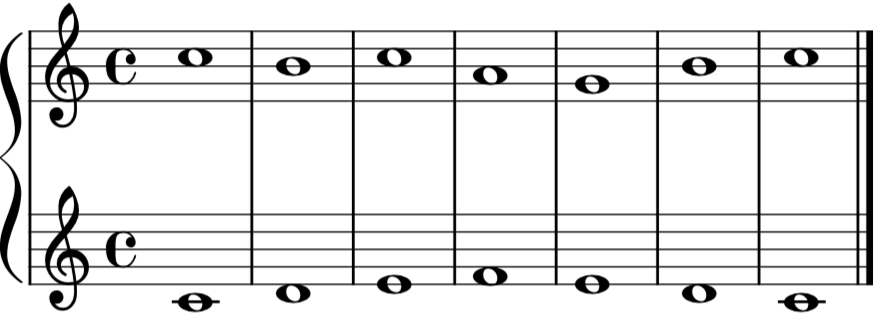
\includegraphics[width=6cm]{fig/fs.png}
    \caption{First Species Counterpoint}
    \Description{First Species Counterpoint}
    \label{fig:fs}
  \end{figure}
}

\newcommand{\MotionCadence}{
  \begin{figure}
    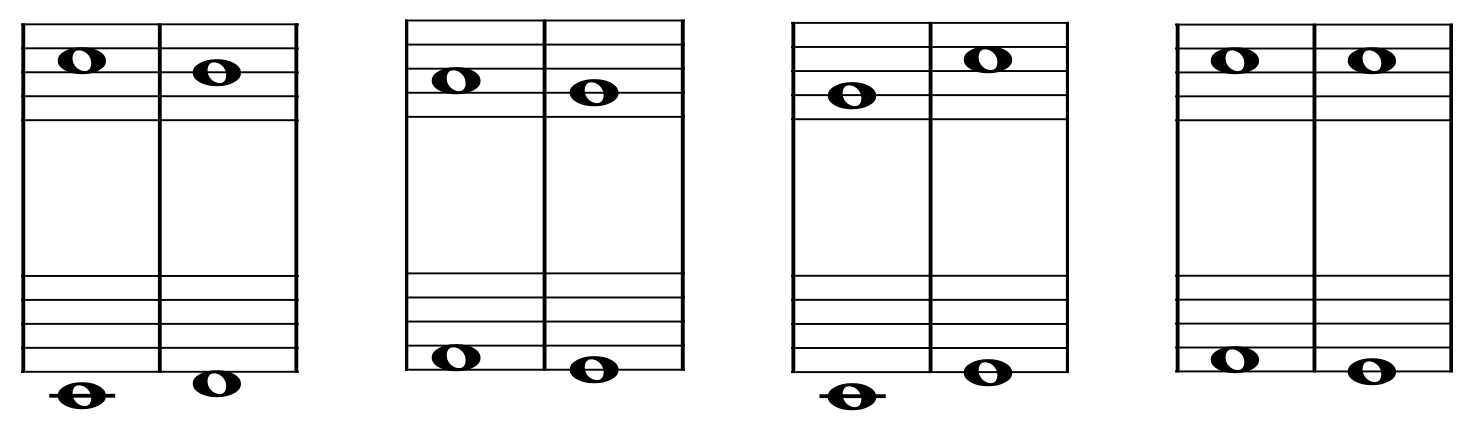
\includegraphics[width=7cm]{fig/motion.png}
    \hspace{1.2cm}
    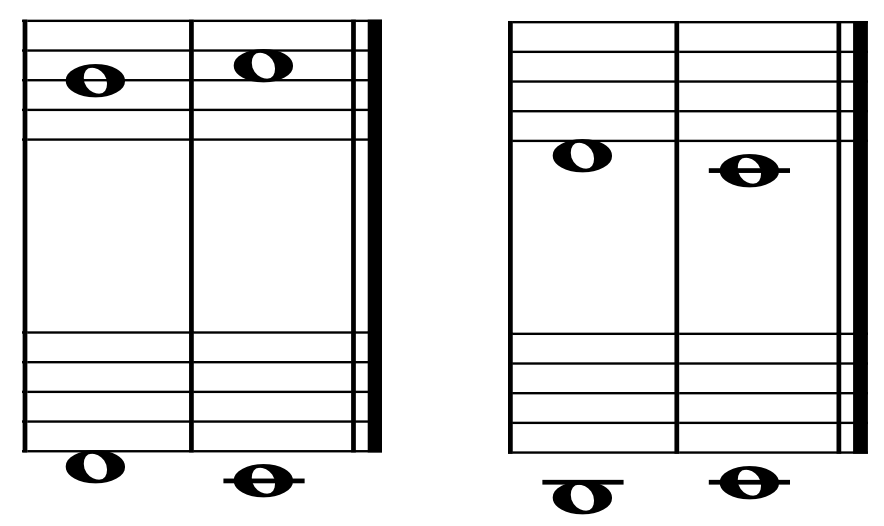
\includegraphics[width=3.33cm]{fig/cadence.png}
    \begin{flushleft}
    \begin{small}
      \hspace{1.2cm} contrary \ \ \ \ \ \ \ \ \,parallel \ \ \ \ \ \ \
      \ \ \ \,similar \ \ \ \ \ \ \ \ \ \ oblique
      %\hspace{1.3cm} paralell-5th \ \ \ similar-8th
    \end{small}
    \end{flushleft}
    \caption{Motion (left) and Cadence (right)}
    \Description{Motion (left) and Cadence (right)}
    \label{fig:motioncadence}
  \end{figure}
}

\renewcommand{\SS}{
  \begin{figure}
    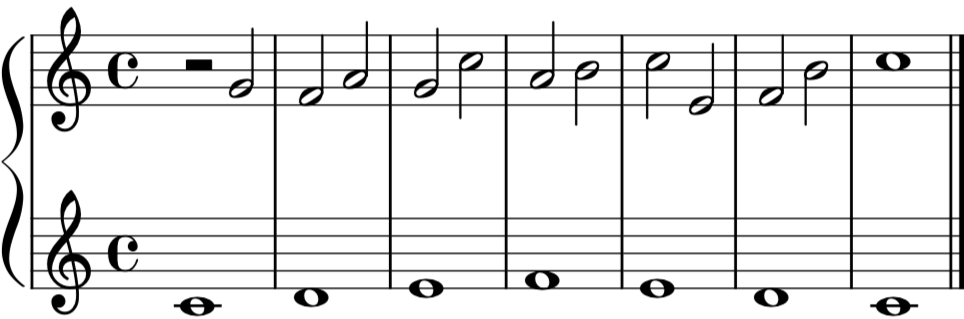
\includegraphics[width=7cm]{fig/ss.png}
    \caption{Second Species Counterpoint}
    \Description{Second Species Counterpoint}
    \label{fig:ss}
  \end{figure}
}

\section{Counterpoint}
\label{sec:cp}

Counterpoint is a technique for combining multiple lines of melodies.
Composing counterpoint is like arranging a song for choir:
we start with a \emph{cantus firmus}, which serves as the base melody,
and compose a counterpoint line above or below the cantus firmus.
When doing this, we must make sure that the whole music sounds
harmonically pleasing, and that the individual melodic lines are
distinguishable to the listener.

In this section, we present an implementation of species counterpoint,
based on the formulation given by \citet{fux-cp}.
The idea is to represent ``good'' counterpoint  as a dependent record,
whose fields encode the musical content as well as proofs that the
counterpoint follows certain rules.
Due to the space limitation, we only show some exerpts of our
implementation; see our anonymous supplementary material
\texttt{Counterpoint.agda} for full details.

\subsection{First Species Counterpoint}
\label{sec:cp:fs}

\FS

First species counterpoint is the simplest variant of counterpoint.
In first species, we set one note against each note in the cantus firmus,
which is required to start with a tonic (the first note of a scale,
such as C in C major) and consist only of whole notes.
Figure~\ref{fig:fs} shows an example of first species counterpoint.
The lower line is the cantus firmus, which we excerpt from a German
song called \emph{Froschgesang} (Frog's song).
The upper line is the counterpoint composed by the second author.

\subsubsection{Representing Music}

In our implementation, we represent each bar as a pitch-interval pair
\texttt{(p ,  i)}, where \texttt{p} is the pitch of a cantus firmus note,
and \texttt{i} is the interval between \texttt{p} and the corresponding
counterpoint note.
We then represent a sequence of bars as a list of pitch-interval pairs,
but with one proviso: we separate the first and last bars from the
middle bars.
Therefore, the Frog's song in Figure~\ref{fig:fs} is represented as a
compound of the following three elements:

\begin{alltt}  
first : PitchInterval -- Pitch \(\times\) Interval
first = (c 5 , per8)

middle : List PitchInterval
middle = (d 5 , maj6) :: (e 5 , min6) :: (f 5 , maj3) ::
         (e 5 , min3) :: (d 5 , maj6) :: []

last : PitchInterval
last = (c 5 , per8)
\end{alltt}

\subsubsection{Representing Rules}

The reason behind our three-part representation of music is that
different parts are subject to different rules, as we detail below.

\paragraph{Beginning}

The beginning of the music should express perfection.
As we saw in Section~\ref{sec:music}, there are three intervals that
are classified as perfect: the 1st (usually called the \emph{unison}),
5th, and 8th.
The first interval of the music must then be one of these intervals.
In our formalization, we implement this rule as the
\texttt{checkBeginning} function, which reports an error
\texttt{not158 i} when the first interval \texttt{i} is an invalid one.
Since Agda does not have exceptions, we turn the error into a
\texttt{Maybe} value by wrapping it around the \texttt{just} constructor.

\begin{alltt}
data BeginningError : Set where
  not158 : PitchInterval \(\rightarrow\) BeginningError
  
checkBeginning : PitchInterval \(\rightarrow\) Maybe BeginningError
checkBeginning pi@(_ , i) =
  if ((i == per1) \(\vee\) (i == per5) \(\vee\) (i == per8))
  then nothing
  else just (not158 pi)
\end{alltt}

\paragraph{Intervals}

The middle bars of the music should maintain consonance of intervals
and independence of melodic lines.
As we saw in Figure~\ref{fig:interval}, consonant intervals include
the unison, 3rd, 5th, 6th, and 8th, and among these, the unison is
clearly an obstacle to distinguishing between the two lines of music.
Therefore, the middle bars must consist only of the latter four intervals.
We encode this rule as the \texttt{checkIntervals} function, which
returns a list of errors corresponding to the occurrences of dissonant
intervals and unisons.

\begin{alltt}
data IntervalError : Set where
  dissonant : Interval \(\rightarrow\) IntervalError
  unison    : Pitch    \(\rightarrow\) IntervalError

intervalCheck : PitchInterval \(\rightarrow\) Maybe IntervalError
intervalCheck (p , i) with isConsonant i | isUnison i
intervalCheck (p , i) | false | _    = just (dissonant i)
intervalCheck (p , i) | _     | true = just (unison p)
intervalCheck (p , i) | _     | _    = nothing

checkIntervals : List PitchInterval \(\rightarrow\) List IntervalError
checkIntervals = mapMaybe intervalCheck
\end{alltt}

\paragraph{Motion}

\MotionCadence

The independence of melodic lines is also affected by \emph{motion},
i.e., the way one interval moves to another interval.
As Figure~\ref{fig:motioncadence} left shows, there are four kinds of motion:
\emph{contrary} (two lines go in different directions),
\emph{parallel} (two lines go in the same direction by the same
distance), \emph{similar} (two lines go in the same direction by
different distances), and \emph{oblique} (one line plays the same note).
It is known that approaching a perfect interval by parallel or similar
motion tends to fuse the melodic lines into one.
To rule out such motion, we define the \texttt{checkMotion}
function, which inspects all pairs of two adjacent intervals (using an
auxiliary function \texttt{pairs}) and returns a list of erroneous patterns.

\begin{alltt}
data MotionError : Set where
  parallel : PitchInterval \(\rightarrow\) PitchInterval \(\rightarrow\) MotionError
  similar  : PitchInterval \(\rightarrow\) PitchInterval \(\rightarrow\) MotionError

motionCheck : PitchInterval \(\rightarrow\) PitchInterval \(\rightarrow\) Maybe MotionError
motionCheck i1 i2 with motion i1 i2 | isPerfect (proj\(\sb{2}\) i2)
motionCheck i1 i2 | contrary | \_     = nothing
motionCheck i1 i2 | oblique  | \_     = nothing
motionCheck i1 i2 | parallel | false = nothing
motionCheck i1 i2 | parallel | true  = just (parallel i1 i2)
motionCheck i1 i2 | similar  | false = nothing
motionCheck i1 i2 | similar  | true  = just (similar i1 i2)

checkMotion : List PitchInterval \(\rightarrow\) List MotionError
checkMotion = mapMaybe (uncurry motionCheck) \(\circ\) pairs
\end{alltt}

\paragraph{Ending}

The ending of the music should express relaxation.
There is a consensus that the unison and 8th are the most stable
intervals, hence the music must end with either of these intervals.
The last interval should also be approached by a \emph{cadence},
a progression that gives rise to a sense of resolution
(Figure~\ref{fig:motioncadence} right).
This in turn suggests that a valid ending requires the middle bars
to be non-empty.
We encode these rules as the \texttt{checkEnding} function, which,
upon finding an invalid ending, reports one of the three possible
errors.

\begin{alltt}
data EndingError : Set where
  not18    : PitchInterval      \(\rightarrow\) EndingError
  not27    : PitchInterval      \(\rightarrow\) EndingError
  tooShort : List PitchInterval \(\rightarrow\) EndingError

endingCheck : PitchInterval \(\rightarrow\) PitchInterval \(\rightarrow\) Maybe EndingError
endingCheck pi1@(pitch p , i) (pitch q , interval 0)  = 
  if ((p + 1 \(\equiv\sp{\mathtt{b}}\) q) \(\wedge\) (i == min3)) then nothing else just (not27 pi1)
endingCheck pi1@(pitch p , i) (pitch q , interval 12) =
  if ((q + 2 \(\equiv\sp{\mathtt{b}}\) p) \(\wedge\) (i == maj6) \(\vee\) (p + 1 \(\equiv\sp{\mathtt{b}}\) q) \(\wedge\) (i == min10))
  then nothing
  else just (not27 pi1)
endingCheck pi1               pi2                     =
  just (not18 pi2)

checkEnding : List PitchInterval \(\rightarrow\) PitchInterval \(\rightarrow\) Maybe EndingError
checkEnding []        \_ = just (tooShort [])
checkEnding (p :: []) q = endingCheck p q
checkEnding (p :: ps) q = checkEnding ps q
\end{alltt}

\subsubsection{Putting Things Together}

Using the encoding of music and rules we have seen so far, we define
\texttt{FirstSpecies}, a record type inhabited by correct first species
counterpoint.
The first three fields of this record type represent the first, middle,
and last bars, respectively.
The last four fields stand for the proofs that the music satisfies all
the required properties.

\begin{alltt}
record FirstSpecies : Set where
  constructor firstSpecies
  field
    firstBar    : PitchInterval
    middleBars  : List PitchInterval
    lastBar     : PitchInterval
    beginningOk : checkBeginning firstBar \(\equiv\) nothing
    intervalsOk : checkIntervals middleBars \(\equiv\) []
    motionOk    : checkMotion (firstBar :: middleBars) \(\equiv\) []
    endingOk    : checkEnding middleBars lastBar \(\equiv\) nothing
\end{alltt}

With this record type, we can show that the counterpoint in
Figure~\ref{fig:fs} is correct, since the music is an inhabitant of
\texttt{FirstSpecies}.

\begin{alltt}
fs : FirstSpecies
fs = firstSpecies first middle last refl refl refl refl
\end{alltt}

\subsection{Second Species Counterpoint}
\label{sec:cp:ss}

\SS

We next discuss a more complex variant of counterpoint, called the
second species.
In second species, we set \emph{two} half notes against every cantus
firmus note.
This gives rise to the distinction between \emph{strong} beats (the
first interval in a bar) and \emph{weak beats} (the second interval).
Figure~\ref{fig:ss} is an example of two-against-one counterpoint,
again composed for the Frog's song.

\subsubsection{Representing Music}

In second species, the first and last bars may have a different structure
from middle bars.
More specifically, it is encouraged to begin the counterpoint line with
a half rest and end with a whole note.
Therefore, in our implementation, we reuse the \texttt{PitchInterval} 
type for the first and last bars, and define a new type
\texttt{PitchInterval2} for middle bars.

\begin{alltt}
first2 : PitchInterval
first2 = (c 5 , per5)

middle2 : List PitchInterval2 -- Pitch \(\times\) Interval \(\times\) Interval
middle2 =
  (d 5 , min3 , per5) :: (e 5 , min3 , min6) :: (f 5 , maj3 , aug4) ::
  (e 5 , min6 , min3) :: (d 5 , min3 , maj6) :: []

last2 : PitchInterval
last2 = (c 5 , per8)
\end{alltt}

\subsubsection{Representing Rules}

The rules for second species counterpoint can be obtained by
tweaking those for first species and adding a few new ones.
Here we go through the rules without showing the corresponding
Agda functions, as they are largely similar to what we defined for
first species.

\paragraph{Beginning}

The beginning of the music may be either the 5th or 8th, but
\emph{not} the unison, as it prevents the listener from recognizing
the beginning of the counterpoint line.
% We restrict the first interval by defining a new error
% \texttt{BeginningError2} and a function \texttt{checkBeginning2}
% that works analogously to \texttt{checkBeginning} for first species.

\paragraph{Strong Beats}

Strong beats in middle bars are constrained by the same rules as in
first species: they must all be consonant, non-unison intervals.
% We encode this restriction as the \texttt{checkStrongBeats}
% function, which, as the \texttt{checkIntervals} function for first
% species, returns a list of found errors.

\paragraph{Weak Beats}

Weak beats are allowed to be dissonant if they are created by a
\emph{passing tone}, i.e., a note in the middle of two step-wise
motions in the same direction (as in bars 4-5 of Figure~\ref{fig:ss}).
They may also be the unison if they are left by step in the opposite
direction from their approach (as in bars 5-6 of Figure~\ref{fig:ss}).
% We implement these rules as the \texttt{checkWeakBeats} function,
% which checks the validity of every three successive beats in the
% middle bars.

\paragraph{Motion}

Parallel and similar motion towards a perfect interval is prohibited
across bars.
% We enforce this rule using the \texttt{checkMotion2} function,
% which uses \texttt{expandPitchIntervals2} to convert a list of
% \texttt{PitchInterval2} into a list of \texttt{PitchInterval}, and
% checks every pair of weak beat and strong beat intervals.

\paragraph{Ending}

The last interval must be the unison or 8th, preceded by an
appropriate interval that constitutes a cadence structure.

\subsubsection{Putting Things Together}

Now we define \texttt{SecondSpecies}, a record type inhabited by
correct second species counterpoint.
As in \texttt{FirstSpecies}, we have three fields holding the musical
content, followed by five fields carrying the proofs of the required
properties discussed above\footnote{
  The auxiliary function \texttt{secondPitch} in \texttt{weakBeatsOk}
  extracts the counterpoint note of a given interval, and
  \texttt{expandPitchIntervals2} turns a list of \texttt{PitchInterval2}s
  into a list of \texttt{PitchInterval}s.
}.

\begin{alltt}
record SecondSpecies : Set where
  constructor secondSpecies
  field
    firstBar      : PitchInterval 
    middleBars    : List PitchInterval2
    lastBar       : PitchInterval 
    beginningOk   : checkBeginning2 firstBar \(\equiv\) nothing
    strongBeatsOk : checkStrongBeats middleBars \(\equiv\) []
    weakBeatsOk   : checkWeakBeats middleBars (secondPitch lastBar) \(\equiv\) []
    motionOk      : checkMotion2 (firstBar ::
                                  (expandPitchIntervals2 middleBars)) \(\equiv\) []
    endingOk      : checkEnding2 middleBars lastBar \(\equiv\) nothing
\end{alltt}

Using \texttt{SecondSpecies}, we can show that the second species
counterpoint in Figure~\ref{fig:ss} is correct.

\begin{alltt}
ss : SecondSpecies
ss = SecondSpecies first2 middle2 last2 refl refl refl refl refl
\end{alltt}

\subsection{Comparison with Previous Work}
\label{sec:cp:comp}

The type-theoretical formalization of counterpoint has first been
attempted by \citet{szamozvancev-welltyped}.
They encode the rule for intervals by declaring a type class
\texttt{ValidHarmInterval} that classifies valid intervals, and then
specifying which instances are invalid using GHC's support for
custom type errors.
They also implement the restriction on motion based on a similar idea.

The availability of the custom type error feature is an advantage of
using Haskell: it allows the rule writer to leverage Haskell's type checker.
We believe that extending Agda with such support would be
beneficial in music formalization and for many other purposes.

More recently, \citet{cong-cp} give an implementation of first
species counterpoint using dependent types in Agda.
Their idea is to represent correct counterpoint as a list-like
datatype, where the base cases enforce a valid ending and the
inductive case guarantees correct uses of intervals and motion
(by means of implicit arguments representing proofs).

Our representation of counterpoint improves on Cong and Leo's
in two ways.
First, while Cong and Leo rely on the Agda type checker to report
errors, we use our own type checker (implemented as the
\texttt{checkXXX} functions) and type errors (defined as the
\texttt{XXXError} datatypes).
This allows us to produce more user-friendly error messages.
Suppose we have replaced the second interval of Figure~\ref{fig:fs} by
an octave (8th) of D, breaking the rule that perfect intervals cannot
be approached by parallel motion.
In our implementation, this causes an error in the \texttt{motionOk}
field, with the following message:

\begin{alltt}
(parallel (c 5 , per8) (d 5 , per8) :: []) != [] of type (List MotionError)
\end{alltt}

\noindent In contrast, Cong and Leo would just report the existence
of an unsolved metavariable \texttt{\_13}, meaning that Agda failed
to construct a proof required by the counterpoint constructor.
Thus, the user would see the following message in the Agda buffer:

\begin{alltt}
\_13 : motionOk (c 5 , per8) (d 5 , per8)
\end{alltt}

\noindent For a non-expert user, it may be difficult to connect
this message to the corresponding musical error.

The second improvement from \citet{cong-cp} is that, instead of
incorporating all the rules into a counterpoint datatype, we define
each rule as a separate function and combining them using a record type.
This makes it easy to switch between strict and relaxed rule sets:
we just need to add or remove certain fields.
It also allows us to reuse some of the rules in a context other than
counterpoint, as we will see in the next section.